\subsection{Score-Based Generative Modeling through Stochastic Differential Equations~--~SDEs}\label{SDEs}

~\citeauthor{song2020score} aim to combine both DDPMs and SGMs (NCSNs) using Stochastic Differential Equations (SDEs). The idea is to create a continuous diffusion process, indexed by time, that transforms a data distribution into a more tractable prior distribution. This is described through the following function by \citeauthor{song2020score}:

\[ dx = f(x, t)dt + g(t)dw, \]

The process is governed by two coefficients: a drift coefficient \( f(x, t) \), governing the deterministic properties of the stochastic process, guiding how data evolves over time, and a diffusion coefficient \( g(t) \), which scales the random noise introduced by Brownian motion \( dw \) (Wiener process) \citep{song2020score}. This Brownian motion represents the random movement of particles in a fluid as they collide with fast-moving molecules in the fluid. 


For generating new samples, a  principle from Anderson \citep{anderson1982313} comes into play. It states that ``the reverse of a diffusion process is also a diffusion process, running backwards in time and given by the reverse-time SDE:\@'' \citep{song2020score}.

\[ dx = \left[ f(x, t) - g{(t)}^2 \nabla_x \log p_t(x) \right] dt + g(t)d\bar{w} \]

This equation by \citeauthor{song2020score} describes the process of recovering data from noise by moving backward in time. ``Once the score of each marginal distribution, \(\nabla_x \log p_t(x) \), is known for all t, we can derive the reverse diffusion process from [the above equation] and simulate it to sample from \(p_0\)'' \citep{song2019SGM}. This score function essentially captures the essence of the data's probability distribution at various stages of noise addition.

\begin{figure}[ht]
  \centering
    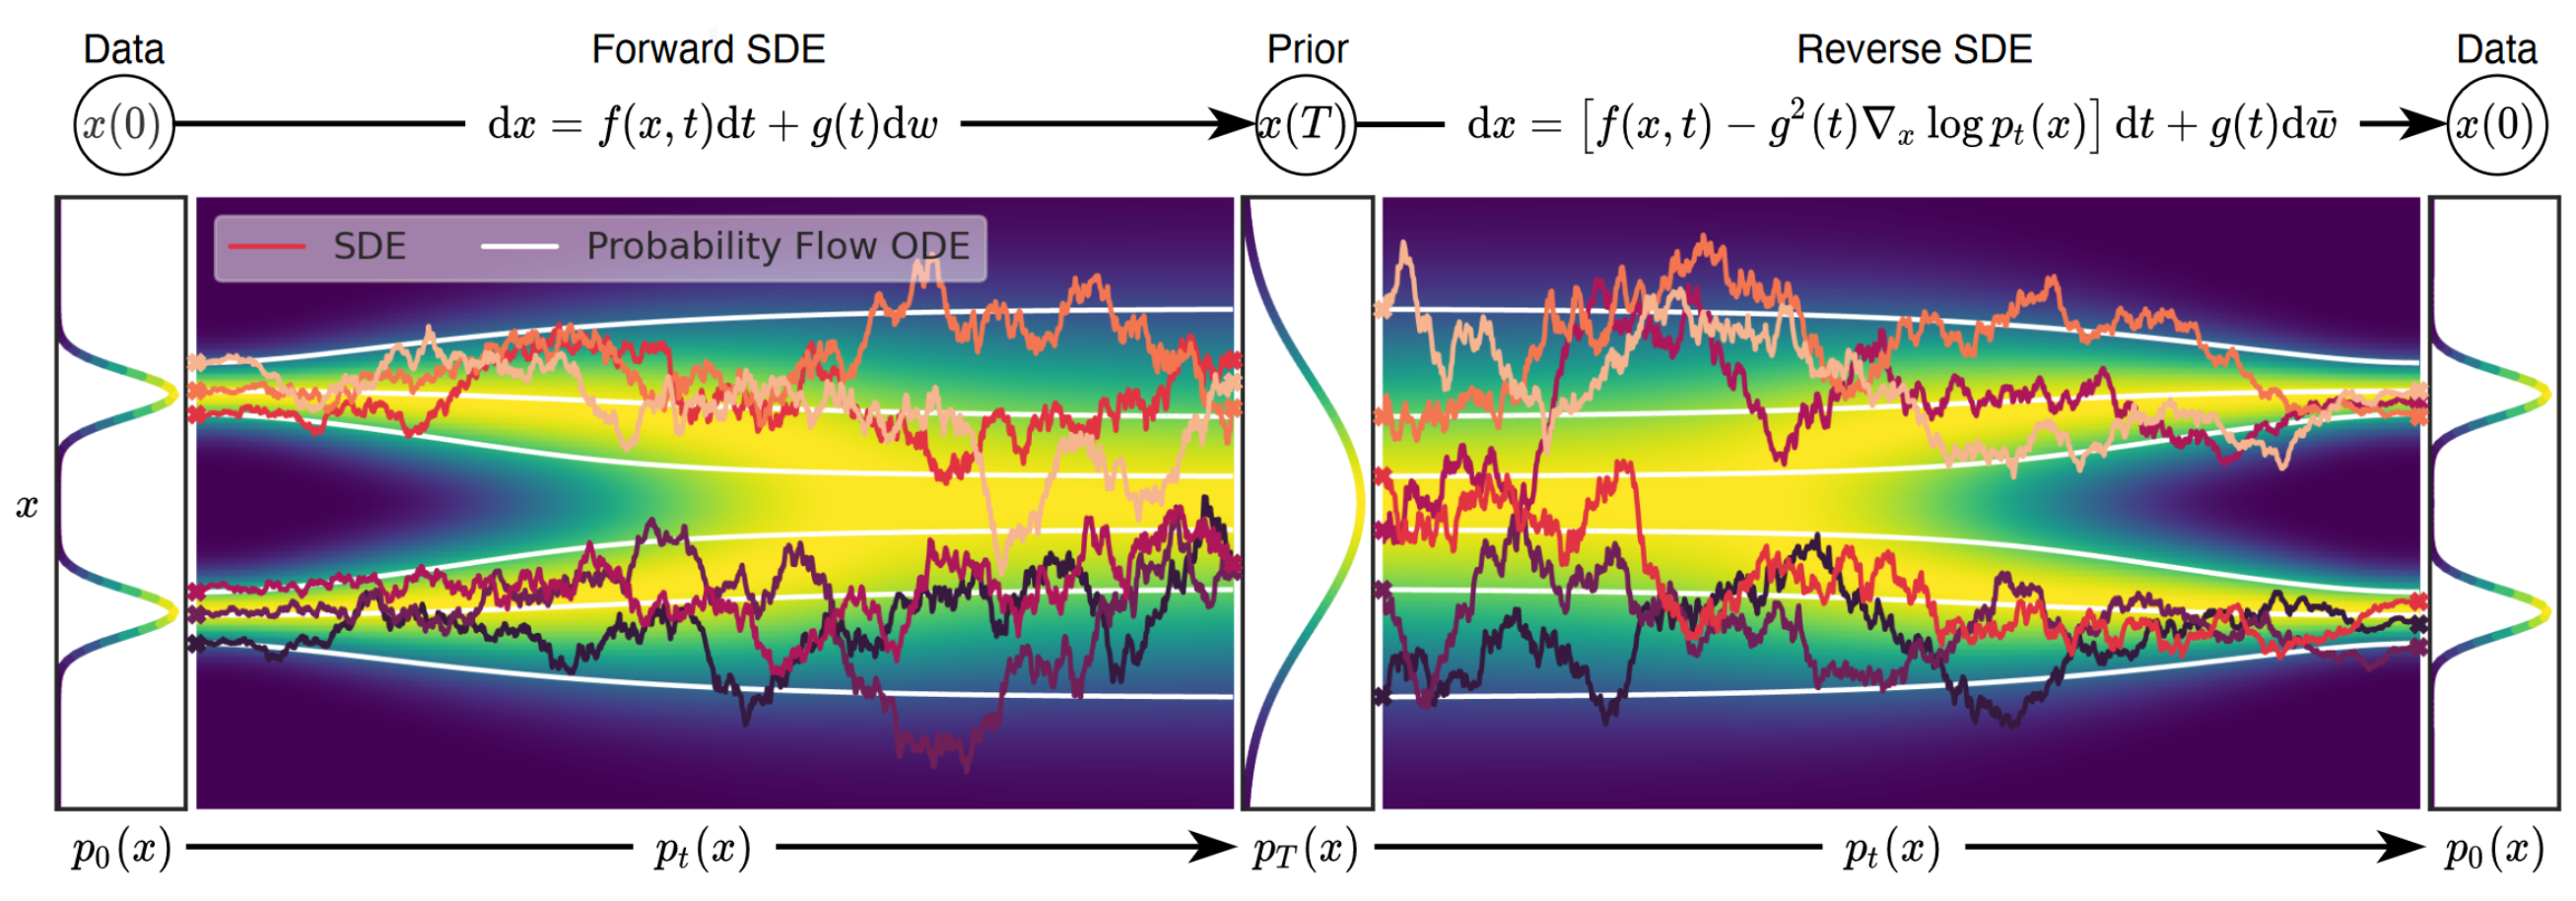
\includegraphics[width=1\columnwidth]{figures/DiffusionModels_SDEs.png}
    \caption{This figure illustrates the two-fold process in score-based generative modeling through SDEs. On the left, the Forward SDE represents the gradual transformation of data into noise, guided by the drift and diffusion coefficients. On the right, the Reverse SDE depicts the process of reconstituting original data from noise, leveraging the known score of each marginal distribution~\citep{song2020score}}\label{fig:DM_SDEs}
\end{figure}

Training a model to accurately estimate the score functions at various noise levels is a fundamental aspect of this process. To achieve this, the model is trained through score matching \citep{hyvarinenScoreMatching}, which involves fine-tuning the model to closely approximate these score functions across a spectrum of noise levels \citep{song2020score}. 


\begin{comment}
[
The training objective, as stated below by \citeauthor{song2020score}, is formulated to find optimal model parameters \( \theta^* \) that minimize the expected discrepancy between the estimated and true scores over time, which are influenced by the noise.

\[
\theta^* = \arg\min_\theta \mathbb{E}_t \left\{ \lambda(t) \mathbb{E}_{x_0} \mathbb{E}_{x_t|x_0} \left\| s_\theta(x_t, t) - \nabla_{x_t} \log p_{0t}(x_t | x_0) \right\|_2^2 \right\}
\]

 The expectations are taken over time and modulated by a time-varying weighting function \( \lambda(t) \). ``With sufficient data and model capacity, score matching ensures that the optimal solution for the above equation, denoted by \(s_{\theta^*}(x, t)\) equals \(\nabla_{x_(t)} \log p_{t}(x)\) for almost all \( x \) and \( t \)'' \citep{song2019SGM}. 
 ]
\end{comment}
 
 The score matching process matches the output of the score network with the true gradient of the log-likelihood over the course of the SDE, enabling the generation of realistic data samples from complex distributions.